\documentclass{beamer}
\usepackage{amsfonts,amsmath,oldgerm}
\usepackage{ragged2e}

\usetheme{sintef}

\newcommand{\testcolor}[1]{\colorbox{#1}{\textcolor{#1}{test}}~\texttt{#1}}

\usefonttheme[onlymath]{serif}

\titlebackground*{assets/background}

\newcommand{\hrefcol}[2]{\textcolor{cyan}{\href{#1}{#2}}}

\title{Aula 03 - Escalabilidade horizontal e Vertical}
\subtitle{2023.1 - LESA 6 -  Laboratório de Escalabilidade de Sistemas}
\course{Tecnologia em Análise e Desenvolvimento de Sistemas}
\author{\href{mailto:luiz.quirino@ifsp.edu.br}{Luiz \textbf{Quirino}}}
\IDnumber{luiz.quirino@ifsp.edu.br}



\begin{document}
\maketitle
\footlinecolor{maincolor}
\section{Introdução}

\begin{frame}{Principais Tipos de Escalabilidade}
	\begin{itemize}
		\item \textbf{Escalabilidade Vertical}
		      \begin{itemize}
			      \item Expansão da rede através da adição de mais energia e memória à unidade de processamento principal.
		      \end{itemize}

		\item \textbf{Escalabilidade Horizontal}
		      \begin{itemize}
			      \item Adição de mais nodes (máquinas) à estrutura de um sistema já existente.
		      \end{itemize}
	\end{itemize}
\end{frame}
\begin{frame}{Importância da Escalabilidade}
	\begin{itemize}
		\item Conceito utilizado ao se buscar aumentar a capacidade de transação de uma plataforma.
		\item Essencial para sustentar o crescimento e a demanda de um sistema.
	\end{itemize}
\end{frame}

\begin{frame}[fragile]{Desenhando...}

	\begin{figure}[H]
		\centerline{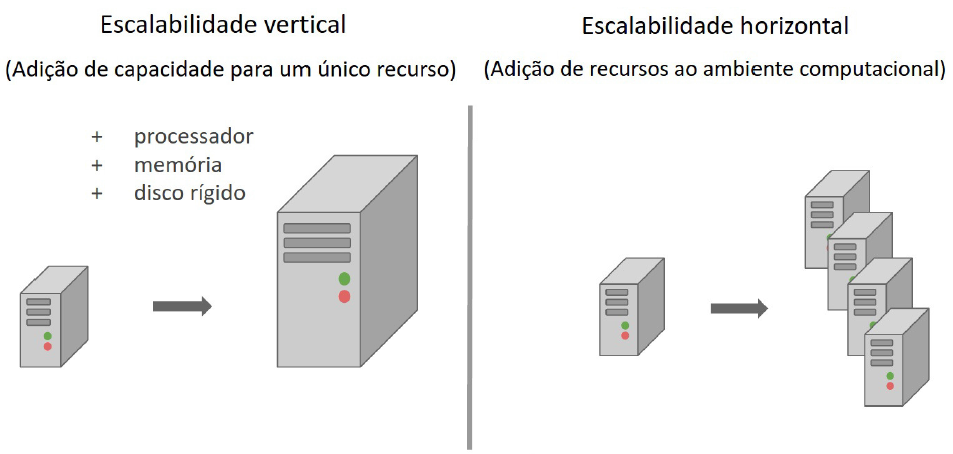
\includegraphics[width=0.8\textwidth]{assets/lesa6/Figura-1.2-Escalabilidade-Vertical-x-Escalabilidade-Horizontal.-Adaptado-de-MARQUESONE-2017.png}}

	\end{figure}
\end{frame}

\section{Expansão de conceitos}

\begin{frame}{Escalabilidade - Horizontal vs. Vertical}
	\begin{itemize}
		\item \textbf{Vertical}: Aumenta a capacidade de um único sistema.
		      \begin{itemize}
			      \item Vantagens: Mais fácil e rápido de implementar.
			      \item Limitações: Tem um limite de eficácia.
		      \end{itemize}

		\item \textbf{Horizontal}: Adiciona mais sistemas ou nodes ao cluster.
		      \begin{itemize}
			      \item Vantagens: Melhora taxa de transferência global.
			      \item Desafios: Leva mais tempo para desenvolver e pode precisar de ajustes de arquitetura.
		      \end{itemize}
	\end{itemize}
\end{frame}

\begin{frame}{Identificando Gargalos}
	\begin{itemize}
		\item Gargalo: Ponto onde a demanda ultrapassa a capacidade, afetando o desempenho.
		\item Examinar gargalos ajuda a determinar qual tipo de escalabilidade é mais adequado.
		\item Necessário para compreender a saúde e performance da plataforma.
	\end{itemize}
\end{frame}
\begin{frame}{Caso Prático - Problema de Memória}
	\begin{itemize}
		\item Situação: Máquina virtual com memória insuficiente para processar transações.
		\item Solução: \textbf{Escalabilidade Vertical}.
		      \begin{itemize}
			      \item Ao adicionar mais memória, a carga é equilibrada.
			      \item Rápida correção para problemas de recursos em um único sistema.
		      \end{itemize}
	\end{itemize}
\end{frame}
\begin{frame}{Caso Prático - Carga de Transação Excessiva}
	\begin{itemize}
		\item Problema: Hardware da plataforma incapaz de lidar com uma alta carga de transações.
		\item Solução: \textbf{Escalabilidade Horizontal}.
		      \begin{itemize}
			      \item Adicionando unidades de processamento adicionais, a demanda é distribuída e gerenciada eficientemente.
		      \end{itemize}
	\end{itemize}
\end{frame}

\begin{frame}{Analogia é minha paixão}

	\begin{columns}
		\column{0.5\textwidth}
		\centering
		
\includegraphics[width=0.3\textwidth]{assets/lesa6/hulk.png} \\
		\textbf{Hulk (Escalabilidade Vertical):}
		\begin{itemize}
			\item Fortalece e expande a si mesmo.
			\item Ex: Como adicionar mais memória ou atualizar a GPU de um servidor.
		\end{itemize}

		\column{0.5\textwidth}
		\centering
		
\includegraphics[width=0.3\textwidth]{assets/lesa6/liga.png} \\
		\textbf{Liga da Justiça (Escalabilidade Horizontal):}
		\begin{itemize}
			\item Une forças com outros super-heróis.
			\item Ex: Como adicionar mais servidores à rede.
		\end{itemize}
	\end{columns}

\end{frame}

\begin{frame}{Analogia é minha paixão - pt2}

    \centering
    
\includegraphics[width=0.3\textwidth]{assets/lesa6/misto.png}
    
    \begin{flushleft}
        \textbf{Escalabilidade horizontal + Vertical = DIAGONAL:}
        \begin{itemize}
            \item Combinação de ambos, vertical e horizontal.
        \end{itemize}
    \end{flushleft}
    
    \end{frame}

    \section{Variantes...}

    \begin{frame}{Escalabilidade Diagonal}\justifying

        Quando você combina escalabilidade vertical com escalabilidade horizontal, você está essencialmente adotando uma abordagem híbrida.
        Esta combinação é frequentemente referida como "escalabilidade diagonal" ou "escalonamento híbrido". A ideia aqui é aproveitar os benefícios de ambos os tipos de escalabilidade para alcançar um desempenho otimizado e flexibilidade para lidar com várias situações de carga.
        
        \end{frame}
        

    \begin{frame}{Benefícios da Escalabilidade Diagonal}

        \begin{itemize}
            \item \textbf{Flexibilidade Máxima}: Adapta-se tanto a picos de carga inesperados (vertical) quanto ao crescimento sustentado ao longo do tempo (horizontal).
            \item \textbf{Otimização de Custo}: Permite investimentos incrementais no hardware existente e na expansão para novos servidores conforme necessário.
            \item \textbf{Resiliência}: Reduz pontos únicos de falha ao combinar o fortalecimento de servidores individuais e a adição de redundância através de mais servidores.
        \end{itemize}
        
        \end{frame}
        \begin{frame}{Considerações sobre o modelo}

            \begin{itemize}
                \item Ao adotar uma estratégia diagonal, as organizações podem se adaptar a diferentes necessidades e situações.
                \item Esta abordagem exige uma gestão cuidadosa para garantir que os recursos sejam utilizados de forma eficiente.
                \item Em última análise, a escolha de vertical, horizontal ou diagonal dependerá das necessidades específicas, dos desafios enfrentados e do orçamento disponível.
            \end{itemize}
            
            \end{frame}
                    
\section{Elasticidade?}

            \begin{frame}{Escalabilidade x Elasticidade} \justifying

                A elasticidade está intimamente ligada à escalabilidade, sendo aquela um atributo desta. Dizer que o sistema é elástico é afirmar que ele tem a capacidade de se adaptar, autonomamente, às mudanças de demanda ocorridas sobre os recursos computacionais. Por exemplo, é o que ocorre quando um e-commerce tem um aumento significativo de acessos e solicitações de forma inesperada, mas o próprio provedor de nuvem se encarrega de reforçar o sistema para atender à nova demanda.
                
                \end{frame}
            
                \begin{frame}{Escalabilidade x Elasticidade} \justifying

                    
                    A elasticidade está intimamente ligada à escalabilidade, sendo aquela um atributo desta. Dizer que o sistema é elástico é afirmar que ele tem a capacidade de se adaptar, autonomamente, às mudanças de demanda ocorridas sobre os recursos computacionais. Por exemplo, é o que ocorre quando um e-commerce tem um aumento significativo de acessos e solicitações de forma inesperada, mas o próprio provedor de nuvem se encarrega de reforçar o sistema para atender à nova demanda.
                    
                    \end{frame}
                

\begin{frame}[fragile]{Imagem do dia}
	\framesubtitle{Computação em nuvem}
	\begin{figure}[H]
		\centerline{
\includegraphics[width=0.4\textwidth]{assets/imagem-do-dia/FxXf1BeWYAACU1r.jpeg}}

	\end{figure}
\end{frame}
\footlinecolor{}

\backmatter
\end{document}
